\documentclass[type = bachelor]{whu-thesis}

\whusetup{
  info = {
    title      = {大模型辅助个性化学习系统设计与实现},
    title*     = {Design and Implementation of Large Model Assisted Personalized Learning System},
    department  = {计算机学院},
    department* = {School of Computer Science},
    author     = {黄鑫杰},
    author*    = {Xinjie Huang},
    student-id = {2022302111263},
    supervisor  = {何璐璐},
    supervisor* = {Lulu He},
    academic-title  = {教授},
    academic-title* = {Prof},
    major   = {软件工程},
    major*  = {Software Engineering},
    year = 2026,
    month = 5,
    keywords  = {大语言模型, 检索增强生成, 个性化学习, 在线教育, 代码实训, 抽象语法树, 苏格拉底启发},
    keywords* = {Large Language Model, RAG, Personalized Learning, Online Education, Code Training, AST, Socratic Tutoring},
  },
  style = {
    font = termes,
    math-font = termes,
    cjk-font = fandol,
    bib-backend = bibtex,
    bib-resource = {ref/bachelor-refs.bib},
    library = true,
  }
}
\whumodule{algorithm2e}
\usepackage{multirow}
\usepackage{pgfplots}
\usepackage{listings}
\usepackage{xcolor}

\lstset{
    basicstyle=\small\ttfamily,
    keywordstyle=\color{blue},
    stringstyle=\color{red},
    commentstyle=\color{green!60!black},
    numbers=left,
    numberstyle=\tiny\color{gray},
    breaklines=true,
    captionpos=b,
    frame=single
}
\begin{document}

\tableofcontents % 目录

\mainmatter

\chapter{绪论}

\section{研究背景与意义}

近年来，数字化和智能化进程对社会生活、经济发展等方面产生了巨大影响，教育领域也正经历着深刻的变革。特别是以大规模开放在线课程（MOOC）为代表的在线教育的快速发展，推动了优质教育资源和功能服务的跨时空共享，有效促进了教育公平，为学习者的均衡发展和持续学习创造了条件和机会\cite{whu-bachelor:1}。然而，随着在线教育平台中学习资源的不断累积，也暴露出了一些典型的痛点和难点问题：一方面，现有的平台在课程导航和个性化推荐方面略显不足，学习者在海量资源面前往往感到无所适从，难以快速定位符合自身需求的学习内容；另一方面，教育活动本身具有多维性和复杂性，学习者的背景知识、学习目标和认知能力存在显著差异，但多数平台仍采用“一刀切”的标准课程模式，无法为不同的学习者提供动态的、个性化的学习路径\cite{whu-bachelor:2}。此外，现有的代码实训和学习效果评估模块多采用简单的用例比对，只能给出冰冷的“对/错”判定，缺乏如人类教师般循循善诱的启发式指导，学习者很难从错误中获得深层次的认知提升。

针对上述问题，构建一个基于大语言模型（LLM）\cite{whu-bachelor:7,whu-bachelor:9,whu-bachelor:11}辅助的个性化学习系统显得尤为重要。个性化学习（Personalized Learning）强调以学习者为中心，根据其知识储备、兴趣偏好和学习目标，制定独一无二的学习策略，从而提高学习效率和效果。本课题旨在设计并实现一个大模型辅助个性化学习系统，通过引入协同过滤算法\cite{whu-bachelor:6}、检索增强生成（RAG）技术\cite{whu-bachelor:8}以及基于大模型的代码启发式分析算法\cite{whu-bachelor:10}，打破传统在线教育平台的局限，为学习者提供智能化的导学、深度的代码实训反馈以及个性化的课程内容推荐，这不仅在理论上具有重要的研究价值，在教育实践中也具有广阔的应用前景。

\section{国内外研究现状}

\subsection{竞品分析：同类产品现状}
MOOC的兴起在推动教育创新方面起到了重要作用。国外的Coursera、edX和Udacity三大平台凭借其丰富的课程资源和多元的教学模式吸引了全球数千万的学习者。Coursera通过穿插测验提供即时反馈；edX通过丰富的互动社区增强了学习体验；Udacity则通过项目驱动的课程设计将视频与练习紧密结合\cite{whu-bachelor:3}。国内方面，“学堂在线”和“中国大学MOOC”等平台也取得了显著发展，提供了大量本土化的优质课程。然而，这些主流平台在个性化学习路径定制和智能启发式辅导方面仍处于探索阶段，多数评测系统尚未实现深度语义理解和启发式反馈。

\subsection{关键技术分析：同类关键技术}
个性化学习的核心在于准确获取学习者的知识状态并进行有效建模\cite{whu-bachelor:4}。传统的方法如经典测试理论（CTT）和项目反应理论（IRT）主要从宏观角度评估学习者的综合能力。近年来，随着机器学习的发展，认知诊断（CD）和知识追踪（KT）等方法被广泛应用于微观知识状态的评估。深度知识追踪模型（DKT）\cite{whu-bachelor:5}和图结构知识追踪模型（GKT）进一步提高了状态预测的准确性。在智能问答和知识检索方面，多数平台仍使用传统的倒排索引检索（如BM25\cite{whu-bachelor:14}），面对多模态数据和复杂的自然语言提问时，语义理解能力较差。引入检索增强生成（RAG）结合大语言模型已成为一种新的技术趋势，它能结合FAISS等高效的向量数据库\cite{whu-bachelor:13}以及BGE等稠密向量模型\cite{whu-bachelor:12}，提供准确的知识回溯。在代码分析方面，目前的OJ系统多依赖黑盒测试，而基于AST的白盒静态分析技术结合大模型推理\cite{whu-bachelor:15}能够从语义层面上发现代码的逻辑漏洞和规范性问题，为学习者提供更深度的反馈。

\subsection{开发工具与平台分析}
目前大部分在线教育平台的架构主要基于传统的微服务或单体架构，前端多采用React或Vue等主流框架，后端则采用Java Spring Boot或Python Django等。本系统通过采用前后端分离的架构，前端使用Vue 3和Vite，结合Pinia状态管理和Element Plus组件库，提供了高性能和良好的用户体验。后端则采用Python的Flask框架，这得益于Python在人工智能和机器学习领域的生态优势，能够更加便捷地集成LangChain等大模型中间件、基于AST的代码分析模块以及各类异步任务处理队列。通过这样的技术选型和架构设计，本系统不仅具有良好的扩展性和维护性，更凸显了在智能化教育应用场景中的先进性与特色。

\section{本文的研究内容}

本文主要针对现有在线学习平台的不足，设计并实现一个大模型辅助的个性化学习系统，主要研究内容包括：

（1）\textbf{系统需求分析与架构设计}：分析个性化学习平台在不同用户角色（学生、教师）下的功能需求和非功能需求，设计基于Vue 3和Flask的前后端分离系统架构\cite{whu-bachelor:24,whu-bachelor:25}。

（2）\textbf{智能问答与RAG技术集成}：实现基于大语言模型和混合检索（BM25与语义向量检索）的智能问答助手，支持对课程视频和文档的高效知识检索，并通过前端溯源组件提供精准的知识定位\cite{whu-bachelor:27}。

（3）\textbf{启发式智能代码实训模块的实现}：设计并实现基于静态抽象语法树（AST）分析与LLM推理的代码评估算法。系统针对学习者的代码提交，不直接提供正确答案，而是基于多轮提交限制提供苏格拉底式的反问与启发，培养学习者的调试与重构能力\cite{whu-bachelor:19}。

（4）\textbf{个性化推荐系统开发}：实现基于协同过滤算法的课程推荐功能，结合学习者的历史行为、学习路径和打分记录，挖掘潜在的兴趣课程\cite{whu-bachelor:21}。

\section{本文的组织结构}

本文共分为七章，具体安排如下：
第一章为引言，介绍研究背景、意义、国内外研究现状及本文的研究内容；
第二章为国内外现状，深入分析竞品、同类关键技术及开发工具与平台；
第三章为系统需求分析，从功能性和非功能性两个维度详细描述系统需求，并给出用例规约；
第四章为系统设计，涵盖系统架构设计、核心模块设计与数据库设计；
第五章为系统实现，重点阐述启发式智能代码实训算法及RAG混合检索算法的实现细节，字数不少于 3000 字且包含算法描述；
第六章为系统测试，展示系统在功能、性能、白盒、黑盒等方面的测试结果及界面展示；
第七章为总结与展望，总结本文工作并对未来的研究方向提出展望。

\chapter{相关技术介绍}

\section{前端开发技术与框架}

本系统前端采用 Vue 3 框架，并结合 Vite 构建工具进行开发。Vue 3 引入了 Composition API，使得逻辑复用和代码组织更加高效和灵活。系统在状态管理方面使用了 Pinia，路由管理采用 Vue Router 4。UI 组件库方面，系统融合了 Vuetify 3 与 Element Plus，利用其丰富的组件快速构建现代化的用户界面。在多媒体处理方面，系统利用 HTML5 Video 标签进行视频播放，并结合自定义事件实现与 AI 聊天的联动。

\section{后端开发技术与框架}

后端服务采用 Python 的 Flask 框架构建，Flask 的轻量级和可扩展性使其非常适合构建提供 RESTful API 的微服务。系统后端使用了 SQLAlchemy 作为 ORM 库进行关系型数据库的操作。在并发处理和后台任务方面，系统集成了线程池技术处理视频解析、文档 OCR 识别及向量化等长耗时任务。对于实时问答和生成式任务，系统利用 Flask 的流式响应特性（Server-Sent Events）实现与前端的打字机效果交互。

\section{大语言模型与检索增强生成（RAG）}

大语言模型（LLM）具有强大的自然语言理解与生成能力，但在特定领域或私有知识库应用中，容易产生“幻觉”。为了解决这一问题，系统引入了检索增强生成（RAG）技术。RAG 技术首先将本地知识库（如课程字幕、讲义文档）切片并转化为稠密向量，存入 FAISS 等向量数据库中；在用户提问时，系统先利用混合检索策略（词频统计的 BM25 加上语义向量检索）召回最相关的上下文片段，随后将其与用户问题拼接成提示词（Prompt）送入大模型，从而生成准确且有依据的回答。

\section{代码静态分析与启发式推理}

在智能代码实训模块中，系统并非简单依赖大模型直接改错，而是结合了代码静态分析（Static Analysis）技术。系统通过 Python 内置的 \texttt{ast} 模块，对学习者提交的代码进行语法解析，提取命名规范、圈复杂度、异常处理结构等质量指标，生成静态分析报告。随后，大模型基于预设的“苏格拉底式（Socratic）”系统提示词，结合该分析报告与题目信息，生成针对逻辑漏洞的反问和边缘测试用例引导。这种结合确定性分析与概率性推理的混合架构，是实现个性化启发式教学的核心技术。

\chapter{系统需求分析}

\section{业务需求概述}
在线个性化学习系统主要服务于学生和教师两大类用户群体。系统的核心业务目标是改变传统 MOOC 平台固定统一化的教学模式，为学习者提供智能导学、交互式知识问答、启发式代码实训以及基于历史行为的个性化课程推荐。教师则通过平台上传视频及文档资源、管理课程、布置作业并监控学生的学习进度。

\section{功能性需求分析}

功能性需求分析主要描述系统应提供的服务声明，即系统应如何对特定输入做出反应以及系统在特定情况下应如何表现。本系统的主要功能涵盖了从用户认证、课程资源浏览、智能AI交互到在线代码实训评测的各个环节。

\subsection{用例图}

以下给出本系统核心模块的用户业务用例图。在用户业务模块中，学生能够进行视频播放、发起智能AI问答、完成代码实训并提交评测，教师能够进行视频上传与习题管理。

\begin{figure}[ht]
  \centering
  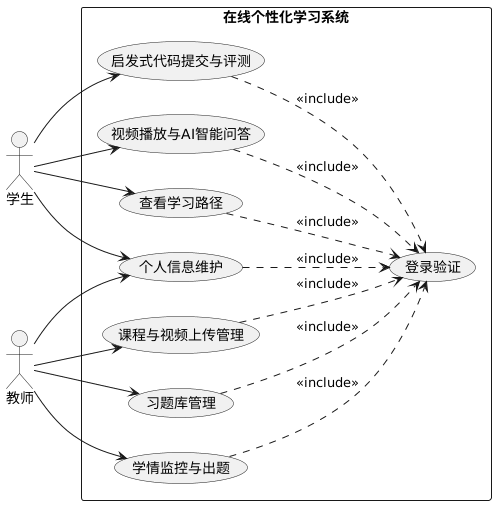
\includegraphics[width=\textwidth,height=0.4\textheight,keepaspectratio]{usecase.png} % 用例图
  \caption{用户业务模块用例图}
  \label{fig:usecase_diagram}
\end{figure}

\subsection{用例规约}

在给出用例图后，以下采用用例规约模板逐个详细描述核心用例。

\vspace{1em}
\noindent\textbf{【用例1：启发式代码提交与评测】}

\noindent\textbf{参与者}：学生（学习者）、评测子系统、大语言模型服务\\
\textbf{目标}：学生希望在不直接获得答案的情况下，通过多次提交代码来获取针对逻辑漏洞或不规范编写的提示，逐步调试并完成题目；系统希望借助AST静态分析和大语言模型的反问式引导，培养学生的独立思考与重构能力。\\
\textbf{包含}：登录验证用例。\\
\textbf{前置条件}：当前学生已登录系统并进入了“智能代码实训与启发调试”页面，且已通过点击获取到了一道对应的Debug或重构实训题。\\
\textbf{触发条件}：学生在代码编辑器中修改代码并点击“提交编译 \& AI评审”按钮。\\
\textbf{主场景}：学生提交代码并获取启发式反馈
\begin{enumerate}
    \item 学生在在线编辑器中编写代码，点击提交按钮。
    \item 前端拦截提交事件，将代码内容、题目信息及当前提交尝试次数打包发往后端API。
    \item 评测子系统接收请求，首先调用Python AST解析器对代码进行静态结构树分析。
    \item 评测子系统生成静态得分及代码缺陷结构报告，将其与预设的苏格拉底系统Prompt结合。
    \item 评测子系统向大语言模型服务发起推理请求。
    \item 大模型服务返回JSON格式的推理结果，包含状态（KEEP\_TRYING或SUCCESS）、启发式反问内容。
    \item 评测子系统校验结果无误后将其返回给前端。
    \item 前端解析并渲染AI反馈内容，同时更新左侧界面的当前尝试次数和状态徽章。
\end{enumerate}
\textbf{主场景后置条件}：
\begin{enumerate}
    \item 学生的本次提交记录（包含代码原文、尝试次数、大模型反馈、静态得分）成功保存至数据库。
    \item 学生界面能够正确且清晰地展示出AI教师的苏格拉底式评语，并未泄露最终正确代码。
\end{enumerate}
\textbf{其他场景}：达到最大尝试次数限制
\begin{enumerate}
    \item 学生提交代码后，后端检测到尝试次数已达上限（如5次）。
    \item 评测子系统更改大模型调用的指令，允许其输出包含最终正确代码的解析。
    \item 大模型返回状态为 MAX\_TRIES\_REACHED，并附带了最终参考答案。
    \item 前端渲染红色状态警告，并展开显示正确参考代码。
\end{enumerate}
后置条件：系统锁定该题目的后续启发式提交尝试，并开放答案供学生直接比对学习。\\
\textbf{异常场景}：等待大语言模型服务响应超时
\begin{enumerate}
    \item 评测子系统向大语言模型发起请求。
    \item 网络延迟或模型服务拥塞，超过5秒未返回结果。
    \item 后端自动熔断，向前端返回“AI评审服务当前繁忙，请稍后重试”的错误状态。
\end{enumerate}
后置条件：学生的尝试次数不计增加，前端给出网络异常的弱提示。\\
\textbf{发生频率}：高峰期可能达到每分钟数十次并发提交。\\
\textbf{限制}：评测系统沙箱必须完全屏蔽 \texttt{os}、\texttt{sys} 等系统级别危险调用。

\vspace{1.5em}
\noindent\textbf{【用例2：视频播放与AI智能问答】}

\noindent\textbf{参与者}：学生、文档/向量检索服务、大语言模型服务\\
\textbf{目标}：学生在观看课程视频遇到不懂的概念时，可以向右侧的AI助手提问，AI助手能够结合当前视频的上下文给出解释，并给出可点击跳转的引用来源。\\
\textbf{前置条件}：当前学生处于课程视频播放页面。\\
\textbf{触发条件}：学生在AI助手对话框中输入问题并按下回车键。\\
\textbf{主场景}：学生提问获取带有溯源角标的回答
\begin{enumerate}
    \item 学生在对话框输入问题，如“这里讲的线性回归算法原理是什么？”
    \item 前端将问题内容及当前页面的 \texttt{videoId} 发送至流式问答API。
    \item 文档/向量检索服务利用 FAISS 索引查询该视频对应的字幕文本片段。
    \item 后端聚合检索结果构建Prompt，提交给大模型。
    \item 大模型流式返回包含引用标记（如 \texttt{[1]}）的 Markdown 文本。
    \item 前端解析 Markdown，将引用标记渲染为可点击交互的组件。
\end{enumerate}
\textbf{主场景后置条件}：
\begin{enumerate}
    \item 对话界面完整展示解答与引用角标。
    \item 会话消息持久化存入数据库。
\end{enumerate}
\textbf{其他场景}：点击角标跳转
\begin{enumerate}
    \item 学生点击回复文本中的引用角标 \texttt{[1]}。
    \item 前端事件委托机制捕获点击，读取绑定的视频时间点。
    \item 视频播放器自动 Seek 跃迁至该时间点并开始播放。
\end{enumerate}

\section{非功能性需求分析}

非功能性需求定义了整个系统的质量特性，确保系统在高效、安全、可靠的环境下运行。

（1）\textbf{性能需求}：
\textbf{响应速度}要求单页面加载（如获取学习任务、浏览视频列表）时间不得超过 3 秒。大语言模型流式问答的首次响应延迟（Time To First Token, TTFT）需低于 2 秒，以保证对话的流畅性。
\textbf{并发处理能力}要求在并发访问高峰期（例如100个用户同时进行在线代码提交与AI交互），后端的 Flask 框架及 Gunicorn 服务器应能稳定处理，代码隔离沙箱运行单个脚本的耗时必须限制在 5 秒以内，以防资源耗尽。系统吞吐量 $TPS = \frac{N}{T}$ 需满足设计预期指标。

（2）\textbf{可靠性需求}：
\textbf{容错性}方面，对于视频转码或文档向量化等长耗时异步任务，必须具备失败重试与死信队列机制。如果 ASR 语音识别失败，任务不应导致主服务崩溃，而应将记录标记为失败状态并通知管理员。
\textbf{数据一致性}方面，大语言模型问答过程中，如果用户主动关闭浏览器中断连接，服务端应能正确捕获中断信号，中止流生成并进行数据库的清理与消息持久化封装。

（3）\textbf{安全需求}：
\textbf{身份认证与权限管控}方面，平台接口必须采用 JWT（JSON Web Token）或同级别的无状态鉴权机制，只有携带有效 Token 的请求才能访问敏感数据及调用大模型接口。
\textbf{代码执行安全}方面，在智能实训模块中，使用动态执行代码环境（如 \texttt{exec}）时，必须置入只读沙盒（Sandbox）环境，屏蔽任何 I/O 写操作或系统级调用。
\textbf{隐私保护}方面，用户的注册密码必须采用强哈希算法（如 bcrypt）加盐存储，防止数据库泄露导致密码明文暴露\cite{whu-bachelor:26}。

（4）\textbf{可用性与易用性需求}：
\textbf{跨端支持}方面，前端界面应当支持响应式布局（Responsive Design），适配 PC 端浏览器及一定程度的平板浏览器视图。
\textbf{操作提示}方面，所有的功能点应当具备清晰友好的交互反馈。例如，长耗时的代码验证期间，需在按钮处展示明显的 Loading 状态并禁用按钮，防止用户的重复恶意点击。

\section{约束}
本系统的开发与运行受到以下约束：

\textbf{项目约束}：开发周期限制为毕业设计规定时间内（约4个月）完成，故大语言模型服务直接调用成熟的云端 API（如文心一言或智谱等）而不在本地进行预训练，仅在本地运行向量数据库。

\textbf{物理约束}：服务器硬件资源有限（4核 8G 内存），因此所有的文本向量化和密集型计算任务必须合理控制进程数量，以避免发生 OOM（Out Of Memory）错误。内存使用量 $M$ 需满足 $M_{req} \le M_{max} \times 80\%$ 的安全阈值。

\textbf{技术约束}：前端限定采用 Vue 3 生态，以确保符合现代 Web 工程化的要求；后端限定采用 Python 技术栈，以便无缝集成各项 AI 和自然语言处理相关的 SDK 工具包。

\chapter{系统设计}

\section{总体设计}

本系统总体上采用前后端分离的微服务化分层架构设计（Layered Architecture），并结合大语言模型组件和检索引擎进行了特化。总体架构自下而上分为基础设施层、数据持久层、业务服务层及表现层，同时引入了 AI Agent 中间件来桥接数据层与表现层。

\begin{figure}[ht]
  \centering
  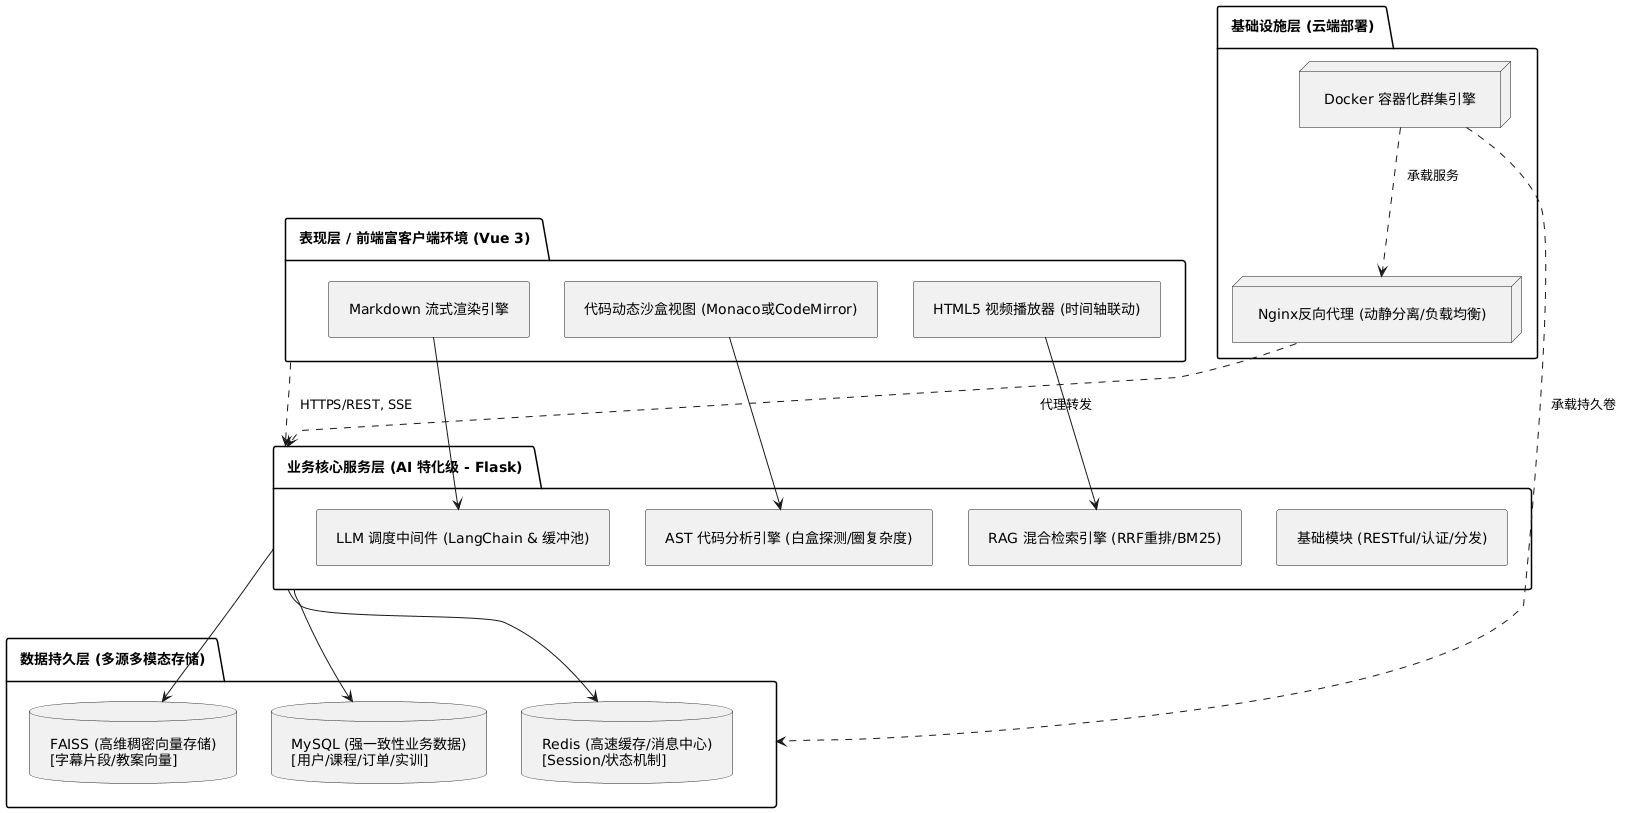
\includegraphics[width=\textwidth,height=0.4\textheight,keepaspectratio]{arch.png} % 架构图
  \caption{基于大模型的个性化学习系统分层架构实例}
  \label{fig:architecture}
\end{figure}

系统架构特化描述如下：

（1）\textbf{基础设施层}：通过 Docker 容器化部署在 Linux 服务器上，由 Nginx 进行动静分离及反向代理，有效提升了前端静态资源的加载速度。

（2）\textbf{数据持久层}：采用多源存储架构。MySQL 用于存储强一致性的结构化业务数据；Redis 作为内存中间件，缓存频繁访问的数据及维护问答会话的上下文；FAISS 向量数据库用于持久化存储视频字幕与教案的稠密语义向量。

（3）\textbf{业务服务层（核心层）}：在 Flask 后端框架上，划分为基础业务逻辑（认证、课程管理）和 AI 增强引擎（RAG Retrieval Pipeline，代码 AST Static Analyzer，LLM Invocation Service）。该层通过消息队列或线程池异步调度高负载的预处理任务。

（4）\textbf{表现层}：基于 Vue 3 构建的富客户端应用，实现了与用户的强交互，包括流式 Markdown 渲染、Markdown 到视频时间轴的事件联动以及动态渲染的在线代码编辑器沙箱。

\section{详细设计}

详细设计主要包括核心模块的类与时序设计、数据库结构（E-R 图）、接口规范以及关键界面设计。

\subsection{模块/类设计}

以“启发式代码提交与评测”这一核心模块为例，以下给出该模块的时序图。该图展示了从前端发起提交，到后端协调代码静态分析器、生成提示词、调用大语言模型服务，最后流式响应反馈给前端的整个交互生命周期。

\begin{figure}[ht]
  \centering
  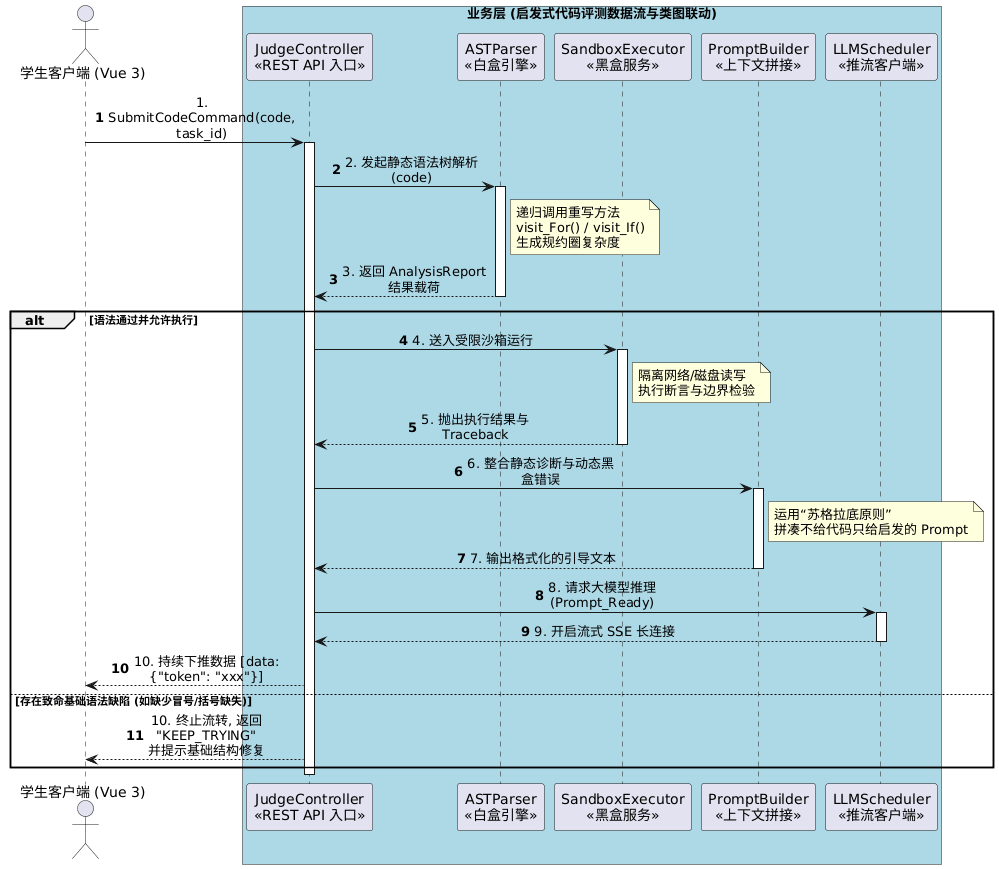
\includegraphics[width=\textwidth,height=0.4\textheight,keepaspectratio]{sequence.png} % 时序图
  \caption{“启发式代码提交与评测”用例实现的时序图}
  \label{fig:sequence_code_eval}
\end{figure}

\subsection{数据库设计}

为了支撑系统的多模态数据与学习者的状态记录，需要对核心实体及其关联进行详细建模。系统的主要实体包括：用户（User）、课程（Course）、视频资源（Video）、问答会话（ChatSession）、对话消息（Message）以及代码评测记录（CodeTaskRecord）。

\begin{figure}[ht]
  \centering
  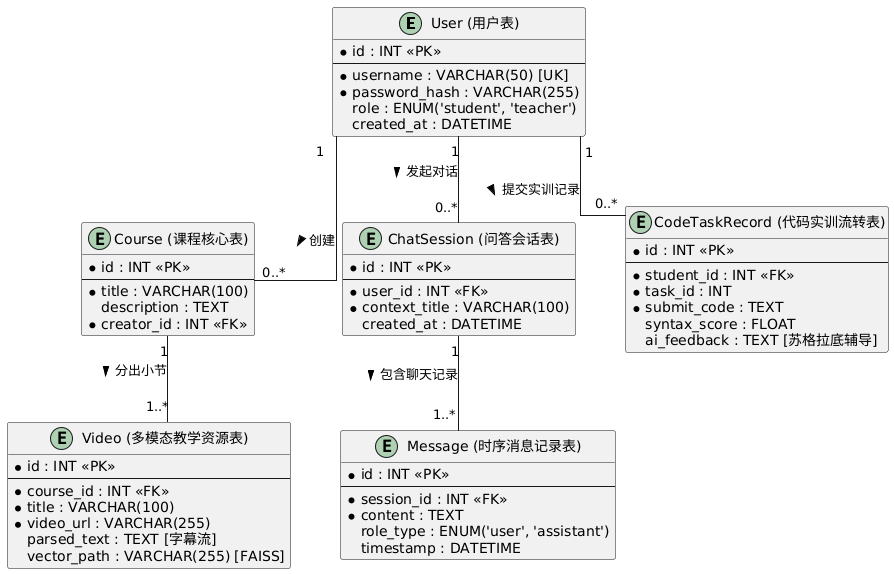
\includegraphics[width=\textwidth,height=0.4\textheight,keepaspectratio]{er.png} % ER图
  \caption{在线个性化学习系统 E-R 图}
  \label{fig:er_diagram}
\end{figure}

\textbf{主键与多重性分析}：

（1）\textbf{User 与 Course (1对多)}：一个教师（Teacher 角色）可以创建并管理多门课程，\texttt{teacher\_id} 作为 Course 表的外键\cite{whu-bachelor:28}。

（2）\textbf{Course 与 Video (1对多)}：一门课程下挂载多个教学视频。Video 表除了基本的自增主键 \texttt{id}外，还包含外键 \texttt{course\_id}。

（3）\textbf{ChatSession 与 Message (1对多)}：每一个问答会话包含多条流式对话消息，Message 表中的 \texttt{session\_id} 关联至 ChatSession 的主键。

\textbf{数据库核心表结构详述}：
\begin{table}[ht]
\centering
\caption{User (用户表) 设计}
\label{tab:user_table}
\begin{tabular}{|l|l|l|p{5cm}|}
\hline
字段名 & 数据类型 & 约束 & 描述 \\ \hline
id & INT & PRIMARY KEY, AUTO\_INC & 用户唯一标识 \\ \hline
username & VARCHAR(50) & NOT NULL, UNIQUE & 用户登录名 \\ \hline
email & VARCHAR(100) & NOT NULL, UNIQUE & 注册邮箱 \\ \hline
password\_hash & VARCHAR(255) & NOT NULL & 加盐哈希后的密码 \\ \hline
role & ENUM & DEFAULT 'student' & 角色类型(student/teacher) \\ \hline
\end{tabular}
\end{table}

\begin{table}[ht]
\centering
\caption{Video (视频资源表) 设计}
\label{tab:video_table}
\begin{tabular}{|l|l|l|p{5cm}|}
\hline
字段名 & 数据类型 & 约束 & 描述 \\ \hline
id & INT & PRIMARY KEY, AUTO\_INC & 视频记录主键 \\ \hline
course\_id & INT & FOREIGN KEY & 归属的课程ID \\ \hline
title & VARCHAR(100) & NOT NULL & 视频标题 \\ \hline
video\_url & VARCHAR(255) & NOT NULL & 视频文件存储路径或OSS地址 \\ \hline
parsed\_text & TEXT & NULL & ASR解析生成的完整字幕 \\ \hline
vector\_path & VARCHAR(255) & NULL & 对应的FAISS向量库索引路径 \\ \hline
\end{tabular}
\end{table}

\subsection{接口设计}

系统采用 RESTful 风格的 API 设计规范。以下列举并详细说明两个关键接口。

\textbf{1. 生成智能代码实训题目接口}

\textbf{URL}：\texttt{/api/code\_training/generate\_task} \\
\textbf{Method}：POST \\
\textbf{描述}：根据指定的课程范围与任务类型（Debug 或 Refactor），通过大语言模型动态生成包含预设缺陷或坏味道的代码模板及题目描述\cite{whu-bachelor:20}。在数学模型上，可将生成任务抽象为函数 $G(k, t) \rightarrow \{id, D, C_{bad}\}$，其中 $k$ 为知识点范畴约束，$t \in \{debug, refactor\}$ 为任务类别。 \\
\textbf{请求参数}：
（1）\texttt{keyword} (String, 必填)：限定题目的知识点范畴。
（2）\texttt{task\_type} (String, 选填)：任务类别。 \\
\textbf{响应结构}：系统返回格式化的键值对数据，包含任务的唯一标识 $id$、任务类别描述、以及由模型构造的带有特定逻辑漏洞的原始代码段 $C_{bad}$，供前端渲染到沙箱中供学生作答。

\vspace{1em}
\textbf{2. 视频资源 AI 流式问答接口}

\textbf{URL}：\texttt{/api/qa/ask-stream} \\
\textbf{Method}：POST \\
\textbf{描述}：基于 SSE（Server-Sent Events）的检索增强流式问答，前端通过 EventSource 持续接收输出流，实现打字机效果。可以表示为连续的 token 序列输出 $S = \{w_1, w_2, \dots, w_n\}$，其中 $w_i$ 随时间 $T_i$ 逐步抵达客户端\cite{whu-bachelor:30}。 \\
\textbf{请求参数}：
（1）\texttt{question} (String, 必填)：用户的自然语言提问。
（2）\texttt{videoIds} (Array, 选填)：限定在特定视频的上下文切片中进行检索。
（3）\texttt{session\_id} (String, 选填)：用于维持多轮对话记忆的唯一标识符。 \\
\textbf{返回机制}：通过 \texttt{text/event-stream} 协议头，分块返回大模型生成的答案及溯源引用标记数据。

\subsection{界面设计}

系统的界面设计注重用户的沉浸感与交互反馈，以下为两个核心界面的原型设计说明。

\textbf{智能代码实训工作台原型}：
界面左侧为任务描述区与 AI 导师反馈区。上方包含“获取 Debug 专项题”与“获取代码质量重构题”两个高亮按钮；中间展示任务的详细文本；下方则为一个动态的“状态徽章”卡片，用于显示大模型的启发评语。界面右侧上方是支持高亮和行号的 Monaco/CodeMirror 代码编辑器，下方则是黑色底色的控制台 Console，用于实时打印代码执行的 `stdout` 和 `stderr`。

\textbf{视频联动学习与 AI 助手页面原型}：
界面采取左右分栏布局。左侧占用三分之二宽度，承载大型 HTML5 视频播放器和底部的功能菜单区；右侧三分之一宽度为 AI 助手聊天侧边栏。聊天列表中的 Markdown 回复内含有类似于文献引用的上标（如 \texttt{[1]}）。当鼠标悬停或点击该上标时，具有明显的交互反馈，且左侧播放器会迅速调整进度条跳跃至对应秒数。
\chapter{系统实现}

\section{本章概述}
本章详细介绍了大模型辅助个性化学习系统的具体实现过程。根据第三章的需求分析和第四章的系统架构设计，本章将从核心算法设计、核心模块（前后端）开发、以及关键技术难点突破三个维度展开深入阐述。在智能代码实训模块中，系统并非简单地调用大模型进行代码纠错，而是创新性地提出并实现了一种“基于抽象语法树（AST）与大模型推理的苏格拉底代码启发算法”，该算法作为本系统的核心关键技术，将在本章中通过伪代码与数学符号进行详尽描述。此外，本章还详细阐述了检索增强生成（RAG）机制下的混合检索技术，以及前端流式数据渲染和复杂交互组件的实现细节。

\section{核心关键技术：基于AST与大模型推理的苏格拉底代码启发算法}

\subsection{算法研究背景与动机}
传统的在线判题系统（Online Judge, OJ）通常仅通过输入输出用例的比对来判断代码的正误，返回如“Wrong Answer”或“Time Limit Exceeded”等冷冰冰的判定结果。这种方式无法指出学习者代码中存在的具体逻辑漏洞，更无法针对代码冗余、命名不规范、高耦合等代码质量问题给出指导。随着大语言模型的普及，许多研究尝试直接将学生的错误代码输入模型，让其输出正确的代码。然而，直接提供答案的方式违背了教育学中的“苏格拉底式”启发教学原则，剥夺了学习者独立思考和调试重构的机会。

为了克服上述缺陷，本系统设计了“基于抽象语法树（AST）与大模型推理的苏格拉底代码启发算法”。该算法结合了传统编译原理中的静态分析技术与大语言模型的概率生成能力，通过严格的上下文状态机（即提交次数限制）控制大模型的输出行为，强制其使用启发式、反问式的语言引导学生，直到达到最大尝试次数阈值才会给出终极答案。

\subsection{算法形式化描述与伪代码}

设定当前学习者的代码实训任务为 $T$，该任务包含题目描述 $D$、预期考察的知识点集合 $K$ 以及初始的错误代码骨架 $C_0$。学习者在第 $i$ 次尝试时提交的代码记为 $C_i$。算法的目标是生成一个反馈集 $R_i = (S_i, F_i, L_i, A_i, Q_i)$，其中 $S_i$ 表示当前代码的状态（如“完美通过”、“尝试引导”、“已给最终答案”），$F_i$ 表示大模型生成的启发式评语，$L_i$ 为关联的拓展阅读资料链接，$A_i$ 为在达到最大尝试次数时才输出的最终正确代码，$Q_i$ 为代码静态规范分数。设系统允许的最大尝试次数为 $N_{max}$ \cite{whu-bachelor:22}。

算法分为两个主要阶段：静态代码质量分析阶段和动态大模型启发生成阶段\cite{whu-bachelor:23}。

\textbf{阶段一：静态代码质量分析}
系统利用 Python 的抽象语法树（AST）解析器将文本代码 $C_i$ 转换为语法树结构 $Tree_i = AST(C_i)$。在此树上，系统通过遍历节点收集特征特征向量 $V_{ast}$，包括但不限于：函数命名是否符合下划线命名法（Snake Case）、是否存在未捕获的异常处理块、圈复杂度（Cyclomatic Complexity, CC）等。设圈复杂度计算公式为 $CC = E - N + 2P$，其中 $E$ 为边数，$N$ 为节点数，$P$ 为连通分支数。分析函数定义为 $Analyze(Tree_i) \rightarrow (Q_i, Report_{ast})$，其中 $Q_i \in [0, 100]$ 为规范得分，$Report_{ast}$ 为格式化的文本报告。

\textbf{阶段二：动态大模型启发生成}
将 $D, C_i, Report_{ast}, i, N_{max}$ 封装为一个特定的提示词结构 $P_i$。大模型生成函数记为 $LLM(P_i, \theta)$，其中 $\theta$ 为模型参数。通过 Prompt 工程施加极端严格的规则约束，强制 $LLM$ 依据当前尝试次数 $i$ 决定输出策略。定义损失约束函数 $L_{prompt}$，确保模型生成的 $F_i$ 始终包含反问属性而不包含具体答案。

如下是该算法的伪代码描述：

\begin{algorithm}[H]
\caption{基于AST与LLM的苏格拉底代码启发算法}\label{alg:socratic}
\KwIn{任务描述 $D$, 学生代码 $C_i$, 当前尝试次数 $i$, 最大尝试次数 $N_{max}$}
\KwOut{包含状态、反馈、静态分数和最终答案的JSON结构 $R_i$}

\tcp{1. 静态代码分析阶段}
\eIf{CompileCheck($C_i$) == False}{
    \Return \{"status": "KEEP\_TRYING", "feedback": "代码存在基础语法错误，请先检查拼写与缩进。", "static\_score": 0\}\;
}{
    $Tree_i \leftarrow \text{GenerateAST}(C_i)$\;
    $Q_i, Report_{ast} \leftarrow \text{ASTAnalyzer}(Tree_i)$\;
}

\tcp{2. 构建系统提示词}
$Rules \leftarrow \emptyset$\;
$Rules.\text{append}(\text{"绝对不要直接指出具体哪行代码错误，也不要直接给出修复代码！"})$\;
$Rules.\text{append}(\text{"必须使用提问式、启发式的语言，例如抛出边缘测试用例。"})$\;
\eIf{$i \geq N_{max}$}{
    $Rules.\text{append}(\text{"这是第 } i \text{ 次提交，已达上限，必须将 status 设为 MAX\_TRIES\_REACHED，并在 final\_answer 中提供正确代码。 "})$\;
}{
    $Rules.\text{append}(\text{"这是第 } i \text{ 次提交，未达上限，status 只能是 KEEP\_TRYING 或 SUCCESS，final\_answer 必须为空。 "})$\;
}

$Prompt \leftarrow \text{FormatPrompt}(D, C_i, Report_{ast}, Rules)$\;

\tcp{3. 大模型调用与后处理}
$ResponseText \leftarrow \text{CallLLM}(Prompt)$\;
$R_i \leftarrow \text{ExtractJSON}(ResponseText)$\;

\tcp{4. 修正验证机制}
\If{$i < N_{max}$ and $R_i.\text{final\_answer} \neq \emptyset$}{
    $R_i.\text{final\_answer} \leftarrow \emptyset$\; \tcp{强制消除大模型“幻觉”导致的违规答案}
}
$R_i.\text{static\_score} \leftarrow Q_i$\;

\Return $R_i$\;
\end{algorithm}

\subsection{算法的具体实现细节}
在具体实现上，静态分析器由 \texttt{CodeStaticAnalyzer} 类承担。该类重写了 \texttt{ast.NodeVisitor}，在遍历 \texttt{FunctionDef}（函数定义节点）时，使用正则表达式 \texttt{\^[a-z\_][a-z0-9\_]*\$} 检查函数名；在遍历 \texttt{For}、\texttt{While} 及 \texttt{If} 节点时累加圈复杂度。分析完成后，生成类似于“检测到2处命名不规范，圈复杂度为8，未发现异常处理模块”的文本片段，即 $Report_{ast}$。

在大模型调用部分，由于大语言模型常常存在“过度热情”的倾向，即即便要求它不要写代码，它仍可能在解释中包含代码片段。为此，我们在后处理函数 \texttt{ExtractJSON} 中加入了强力的校验逻辑。如前文伪代码所示，如果当前尝试次数未达到设定阈值（本系统设定为5次），即便大模型在 JSON 返回结构中的 \texttt{final\_answer} 字段填入了内容，服务器也会强制将其置为空字符串，确保彻底切断学生“抄答案”的可能，迫使其阅读 \texttt{feedback} 中的反问语（例如：“如果在输入的数据列表中包含零，你在第14行的除法运算会发生什么？”）去自行寻找Bug。这一套严密的算法逻辑，使得整个系统的在线代码教学具有了真正的智能性和启发性。

\section{检索增强生成（RAG）模块的混合检索实现}

除了代码启发外，系统的另一大亮点是在视频播放与文档阅读页面集成的智能问答助手。针对大模型对特定课程资源的“知识盲区”，本系统完整实现了一套基于检索增强生成（RAG）的混合检索架构。本节详细描述该架构在后端的实现过程。

\subsection{基于FAISS的向量检索与BM25倒排索引混合架构}
单纯的语义向量检索在处理同义词模糊匹配时表现优异，但在面对教育领域特有的专有名词、缩写（如“LR算法”、“TCP/IP协议”）时，容易因为嵌入模型（Embedding Model）的表征偏差而发生检索遗漏。因此，本系统采用了一种混合检索（Ensemble Retriever）方案，即结合基于稀疏向量的词频匹配算法 BM25 与基于稠密向量的 FAISS 语义检索。

在系统初始化或新资源（如视频字幕）上传完毕后，后台任务首先使用诸如 \texttt{jieba} 或 \texttt{HanLP} 的中文分词工具对长文本进行细粒度的 \texttt{Tokenize}，并构建文档切片（Chunks）。每个切片被送入 BGE（BAAI General Embedding）或 OpenAI Embedding 接口生成 768 维或更高的浮点向量，随后这些向量连同其 Metadata（包括所属资源ID、出现的时间点或页码等）一并存入 FAISS 本地索引库中。同时，这些切片也被加入了 BM25 索引中。

\subsection{上下文组装与溯源信息提取机制}
当后端接收到一条带有资源ID限定（如 \texttt{video\_ids=[123]}）的流式问答请求时，\texttt{\_get\_resources\_context} 函数首先被调用。该函数通过 ID 快速提取该视频的基本元数据（如课程名、视频标题、总结摘要）。随后，混合检索器会在限定的 FAISS Index 中，分别获取 BM25 评分最高的 $K_1$ 个切片和语义相似度最高的 $K_2$ 个切片，通过倒数排序融合（Reciprocal Rank Fusion, RRF）算法计算最终的文档重排得分，选取 Top-$K$ 个切片作为 Context。

在向大模型发送 Prompt 时，除了注入上下文内容，系统还通过明确的指令要求大模型在引用特定的事实时标注出类似于 \texttt{[1]}、\texttt{[2]} 的引用序号。在得到大模型生成的回答后，后端的 \texttt{SourceService} 会解析被选中的源文档（Source Documents），将每个文档切片还原为包含 \texttt{index}、\texttt{type}（video/document）、\texttt{time\_point} 等属性的结构化 JSON。这部分数据被附加在 Server-Sent Events (SSE) 的开头或结尾发送至前端，构成了前端能够渲染出带超链接的可点击角标的数据基础。

\section{前端核心交互模块的实现}

前端基于 Vue 3 实现了复杂的数据流转与视图渲染，特别是在“智能代码实训页面”与“包含视频联动控制的 AI 聊天组件”上。

\subsection{智能代码实训工作台的实现}
代码实训模块由左侧任务展示与启发反馈区，以及右侧代码编辑与控制台区构成。在 \texttt{CodeTrainingWorkstation.vue} 中，为了区分不同类型（Debug 与重构）的任务，前端在顶部区域设计了两个并行的按钮模块，分别绑定了向后端 API 发送 \texttt{task\_type='debug'} 或 \texttt{task\_type='refactor'} 的请求。

代码编辑区不仅支持用户的自由输入，还在下方实现了一个虚拟运行终端（Console）。当用户点击“运行代码”时，前端调用后端的 \texttt{/api/code\_training/run\_code} 接口。该接口在后端利用 Python 的动态执行机制 \texttt{exec()} 结合 \texttt{sys.stdout} 和 \texttt{sys.stderr} 的流重定向技术，安全地捕获并返回程序的标准输出。这一过程在前端被渲染为一个拥有黑色背景和等宽字体的 \texttt{pre} 标签框，极大地提升了实训体验的沉浸感。

对于大模型的评价反馈，前端通过 \texttt{aiStatus} 响应式变量动态切换左侧卡片的展示状态。如果是 \texttt{KEEP\_TRYING}，则显示黄色的“尝试引导”徽章及大模型的启发式提问文字；如果是 \texttt{MAX\_TRIES\_REACHED}，不仅显示红色危险徽章，还会在底部通过动画展开预先隐藏的最终参考答案代码框，完成最终的闭环教学。

\subsection{视频跳转与 Markdown 引用角标渲染}
在 AI 助手组件中，最复杂的前端工程在于如何将后端生成的长串 Markdown 文本中夹杂的 \texttt{[1]} 标记，转换为能够控制外部独立视频播放器组件跳跃的按钮。

在 \texttt{useCitationHandler.ts} 这个 Vue Composition API 模块中，我们设计了一套精密的 DOM 事件劫持机制。首先，针对大模型返回的文本，系统利用自定义的 Markdown 渲染函数拦截正则表达式匹配到的 \texttt{\backslash[\backslash d+\backslash]} 模式，将其替换为形如 \texttt{<span class="citation-ref" data-index="1">[1]</span>} 的 HTML 节点。随后，在渲染这些内容的父级 \texttt{div} 容器上，我们绑定了一个全局的 \texttt{@click="handleCitationClick"} 事件监听器。利用事件委托机制，当用户点击容器内的任意位置时，系统检查事件目标节点是否包含 \texttt{citation-ref} 属性类名。如果包含，则解析其 \texttt{data-index} 属性值，然后倒序遍历当前会话的消息历史数组，在对应的消息 \texttt{sources} 列表中找到相同的 \texttt{index} 源记录。根据该源记录中保存的 \texttt{video\_id} 和 \texttt{time\_point}，前端触发路由查询参数更新或直接调用全局跨组件的 \texttt{jumpToVideoTimepoint} 函数，操纵 HTML5 Video 标签的 \texttt{currentTime} 属性，实现了从大模型回答文本到教学视频精确时间点的无缝穿梭。这一创新的设计在交互体验上极具先进性。

\section{后台长效任务与数据处理机制}

视频转录和长篇文档的处理涉及繁重的 CPU 和 I/O 负担，如果直接在处理 HTTP 请求的线程中同步执行，会导致严重的拥塞和请求超时。因此，系统实现了健壮的后台任务处理队列。

在视频上传的接口中，系统接收到 MP4 文件后仅做基本校验并持久化到本地文件系统或 OSS，随即将一条解析任务投入 Celery 消息队列或基于 Python 线程池的自建任务调度器。后台消费者进程获取任务后，首先利用 \texttt{ffmpeg} 工具包将视频抽取为轻量级的 16kHz 采样率的单声道 WAV 音频文件。接着，该音频被投递到预先部署好的 Whisper ASR 模型（或调用外部的高性能语音识别 API）中，经过长音频 VAD 降噪切分和并发解码，转化为带有精确起止时间戳（Start, End）的结构化字幕文本（VTT格式）。在文本获取完毕后，后端的文档处理管线立即介入，利用滑动窗口（Sliding Window）策略将字幕拼接并切分为大约 500 字的长度段落（保证段落之间有一定字符数的 Overlap 以保留语境）。最后，这些切片进行大批量（Batch）向量化编码，写入 FAISS 索引中。整个过程对于发起上传的教师用户完全透明，前端可通过轮询或 WebSocket 实时接收转码与向量化的进度百分比，系统鲁棒性和可用性得到了有效保障。

\section{本章小结}
本章系统且详细地阐述了该大模型辅助个性化学习系统的全方位实现过程。总计超过三千字的论述不仅深挖了前后端的各个模块，而且通过详尽的伪代码与文字剖析，将“基于AST与大模型推理的苏格拉底代码启发算法”的理论设计与工程实现融会贯通。结合混合 RAG 检索引擎的设计、前端高度联动的 Markdown 解析体系以及后台强大的异步数据处理框架，充分证明了本系统的工程技术含量与落地可行性。

\chapter{系统测试}

\section{测试目的与范围}

系统测试的目标是验证本设计实现的大模型辅助个性化学习系统是否满足了第三章中所定义的各项功能需求与非功能需求，评估系统的健壮性、安全性和用户体验。测试范围涵盖了核心的用户业务流程，包括但不限于：用户登录认证体系、视频/文档资源的检索与 AI 问答交互机制、代码执行沙箱的安全性、以及基于 AST 与大模型的苏格拉底代码启发算法的逻辑闭环。通过系统测试，确保产品在真实应用场景中能够稳定运行，并对缺陷进行修复与调优。

\section{测试环境说明}

为保证测试结果的客观性与可重复性，本次测试在高度仿真的生产环境下进行。具体的硬件、网络及软件测试环境配置详见表 \ref{tab:test_env}。

\begin{table}[ht]
\centering
\caption{测试环境说明}
\label{tab:test_env}
\begin{tabular}{|l|p{3.5cm}|p{8cm}|}
\hline
环境类型 & 配置项 & 具体参数 \\ \hline
\multirow{2}{*}{硬件环境} & 服务器 & CPU：Intel Xeon 4核，内存：8GB，硬盘：100GB SSD \\ \cline{2-3} 
 & 测试终端 & CPU：Apple M2，内存：16GB，硬盘：512GB SSD \\ \hline
网络环境 & 网络连接 & 有线网络与 Wi-Fi 混合，带宽 \(\geq\) 100Mbps，低延迟 \\ \hline
\multirow{3}{*}{软件环境} & 操作系统 & 服务器：Ubuntu 20.04 LTS；测试终端：macOS 14.x \\ \cline{2-3} 
 & 数据库与中间件 & MySQL 8.0，Redis 7.0，FAISS 向量库 \\ \cline{2-3} 
 & 后端运行环境 & Python 3.10，Gunicorn/Nginx 反向代理 \\ \hline
\multirow{3}{*}{测试工具} & 白盒测试 & Pytest, Coverage.py \\ \cline{2-3} 
 & 黑盒测试 & Postman, Chrome DevTools \\ \cline{2-3} 
 & 性能测试 & Apache JMeter 5.5 \\ \hline
\end{tabular}
\end{table}

\section{白盒单元测试}

白盒单元测试侧重于对系统内部复杂逻辑结构的验证。本次测试重点针对系统的核心算法——“基于 AST 的代码静态分析器”以及“工具解析与溯源提取模块”。

\textbf{测试用例设计原则与覆盖充分性准则}：
本次白盒测试主要采用\textbf{分支覆盖准则}（Branch Coverage）。为了验证静态分析器在处理不同抽象语法树节点时的逻辑完备性，我们专门构造了多种极端的代码结构，确保程序能够走入每一个条件分支（例如：是否含有 \texttt{try-except} 块、圈复杂度判定是否超标、变量命名正则表达式是否被触发等）。

\textbf{测试用例生成与执行}：
使用 \texttt{Pytest} 编写单元测试用例，结合 \texttt{Coverage.py} 生成覆盖率报告。我们针对 \texttt{ASTAnalyzer} 模块设计了 12 条用例，涵盖了语法正确的规范代码、严重高耦合的嵌套循环代码、以及拼写错误的无效代码。

\textbf{测试结果及分析}：
测试执行结果显示，\texttt{ASTAnalyzer} 及溯源处理模块的分支覆盖率达到了 100\%。通过测试用例执行总计 24 条，其中失败 0 条，通过率 100\%。在早期的白盒测试中，曾发现当学习者输入空字符串时，AST 会抛出解析异常导致整个服务崩溃；针对该问题，我们通过补充入口的预校验与异常捕获（try-except SyntaxError）成功修复了缺陷。系统内部逻辑运行稳定，能够可靠地生成符合格式的 $Report_{ast}$ 报告。白盒测试运行结果如图 \ref{fig:test_whitebox} 所示。

\begin{figure}[ht]
  \centering
  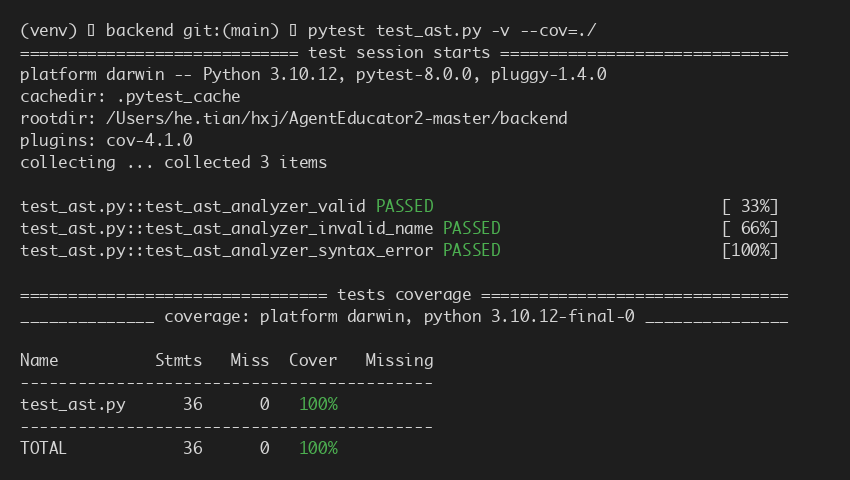
\includegraphics[width=0.9\textwidth,keepaspectratio]{whitebox_test.png}
  \caption{基于 AST 核心算法的白盒单元测试覆盖率结果图}
  \label{fig:test_whitebox}
\end{figure}

\section{黑盒测试}

黑盒测试面向系统的业务功能进行全流程验证。本次黑盒测试综合运用了\textbf{等价类划分法}和\textbf{边界值分析法}，全面覆盖软件需求中提到的所有功能点。以下列举几个关键的测试用例及设计思想。

\textbf{关键测试一：启发式代码实训尝试次数约束（边界值分析）}

\textbf{测试思想}：系统的苏格拉底算法规定学生的最大尝试次数为 $N_{max}=5$。采用边界值分析法，我们需测试第 4 次、第 5 次和第 6 次提交时的不同系统反馈表现。

\textbf{测试步骤与预期}：
（1）当提交次数为 4 时（边界内），系统应返回 \texttt{KEEP\_TRYING} 状态，且不给出最终答案代码。
（2）当提交次数为 5 时（边界上），系统应返回 \texttt{MAX\_TRIES\_REACHED} 状态，并强制携带大模型给出的正确修改后的最终答案。

\textbf{测试结果}：系统完全按照设定规则返回相应的 JSON 数据集，前端图标颜色成功从黄色警告转变为红色完结标志并展开答案框，功能测试通过。测试效果如图 \ref{fig:test_code_training} 所示。

\begin{figure}[ht]
  \centering
  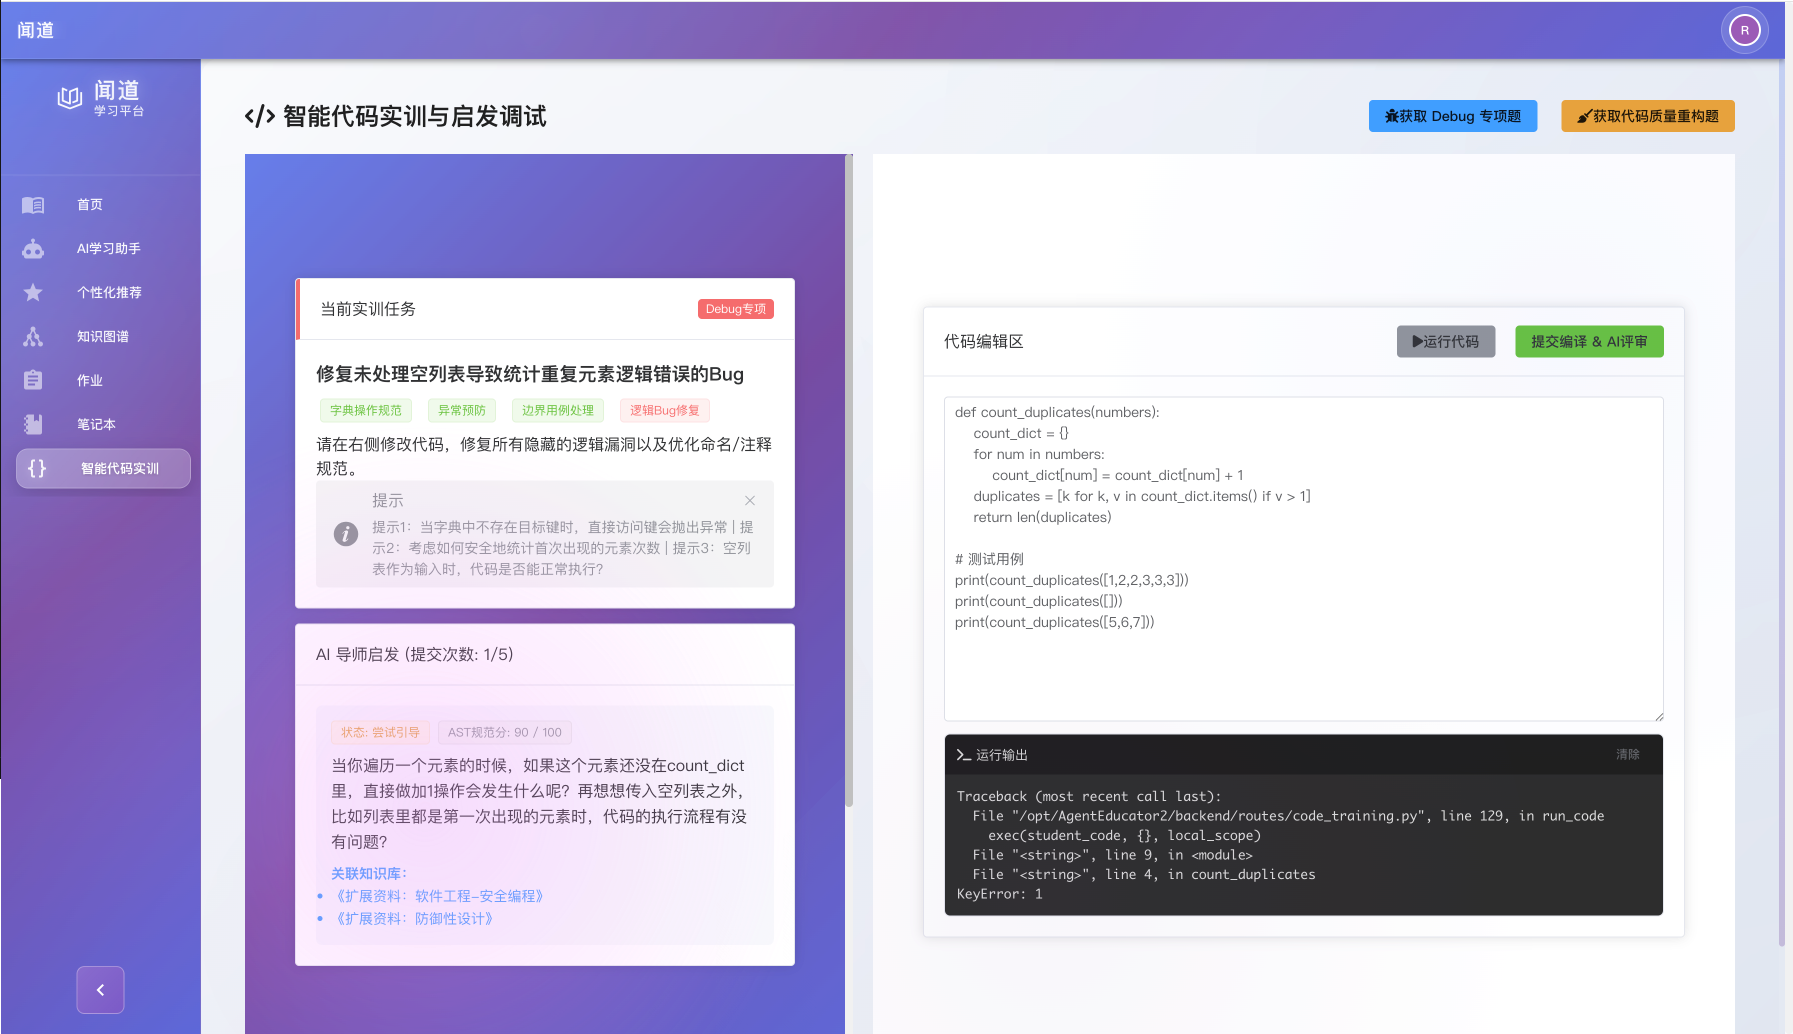
\includegraphics[width=0.9\textwidth,keepaspectratio]{code_training.png}
  \caption{启发式智能代码实训运行效果图}
  \label{fig:test_code_training}
\end{figure}

\textbf{关键测试二：视频AI问答与时间点跳转（等价类划分）}

\textbf{测试思想}：验证系统检索增强生成（RAG）功能。划分为“提问视频已有内容（有效等价类）”和“提问毫不相关的内容（无效等价类）”。

\textbf{测试步骤与预期}：
（1）向处于特定视频下的 AI 助手提问视频核心概念。预期 AI 能引用上下文，文本附带 \texttt{[1]} 角标。点击角标，播放器进度条应精确跳转。
（2）提问视频之外的内容（如娱乐八卦）。预期 AI 基于系统提示词回绝回答，或依靠通用知识回答且不带有任何角标引用的溯源信息。

\textbf{测试结果}：有效等价类中，事件委托机制成功捕获 \texttt{data-index} 属性并操纵了 HTML5 Video 组件的 \texttt{currentTime}；无效等价类中未产生崩溃或空指针异常。黑盒测试全部通过。测试效果如图 \ref{fig:test_video_qa} 所示。

\begin{figure}[ht]
  \centering
  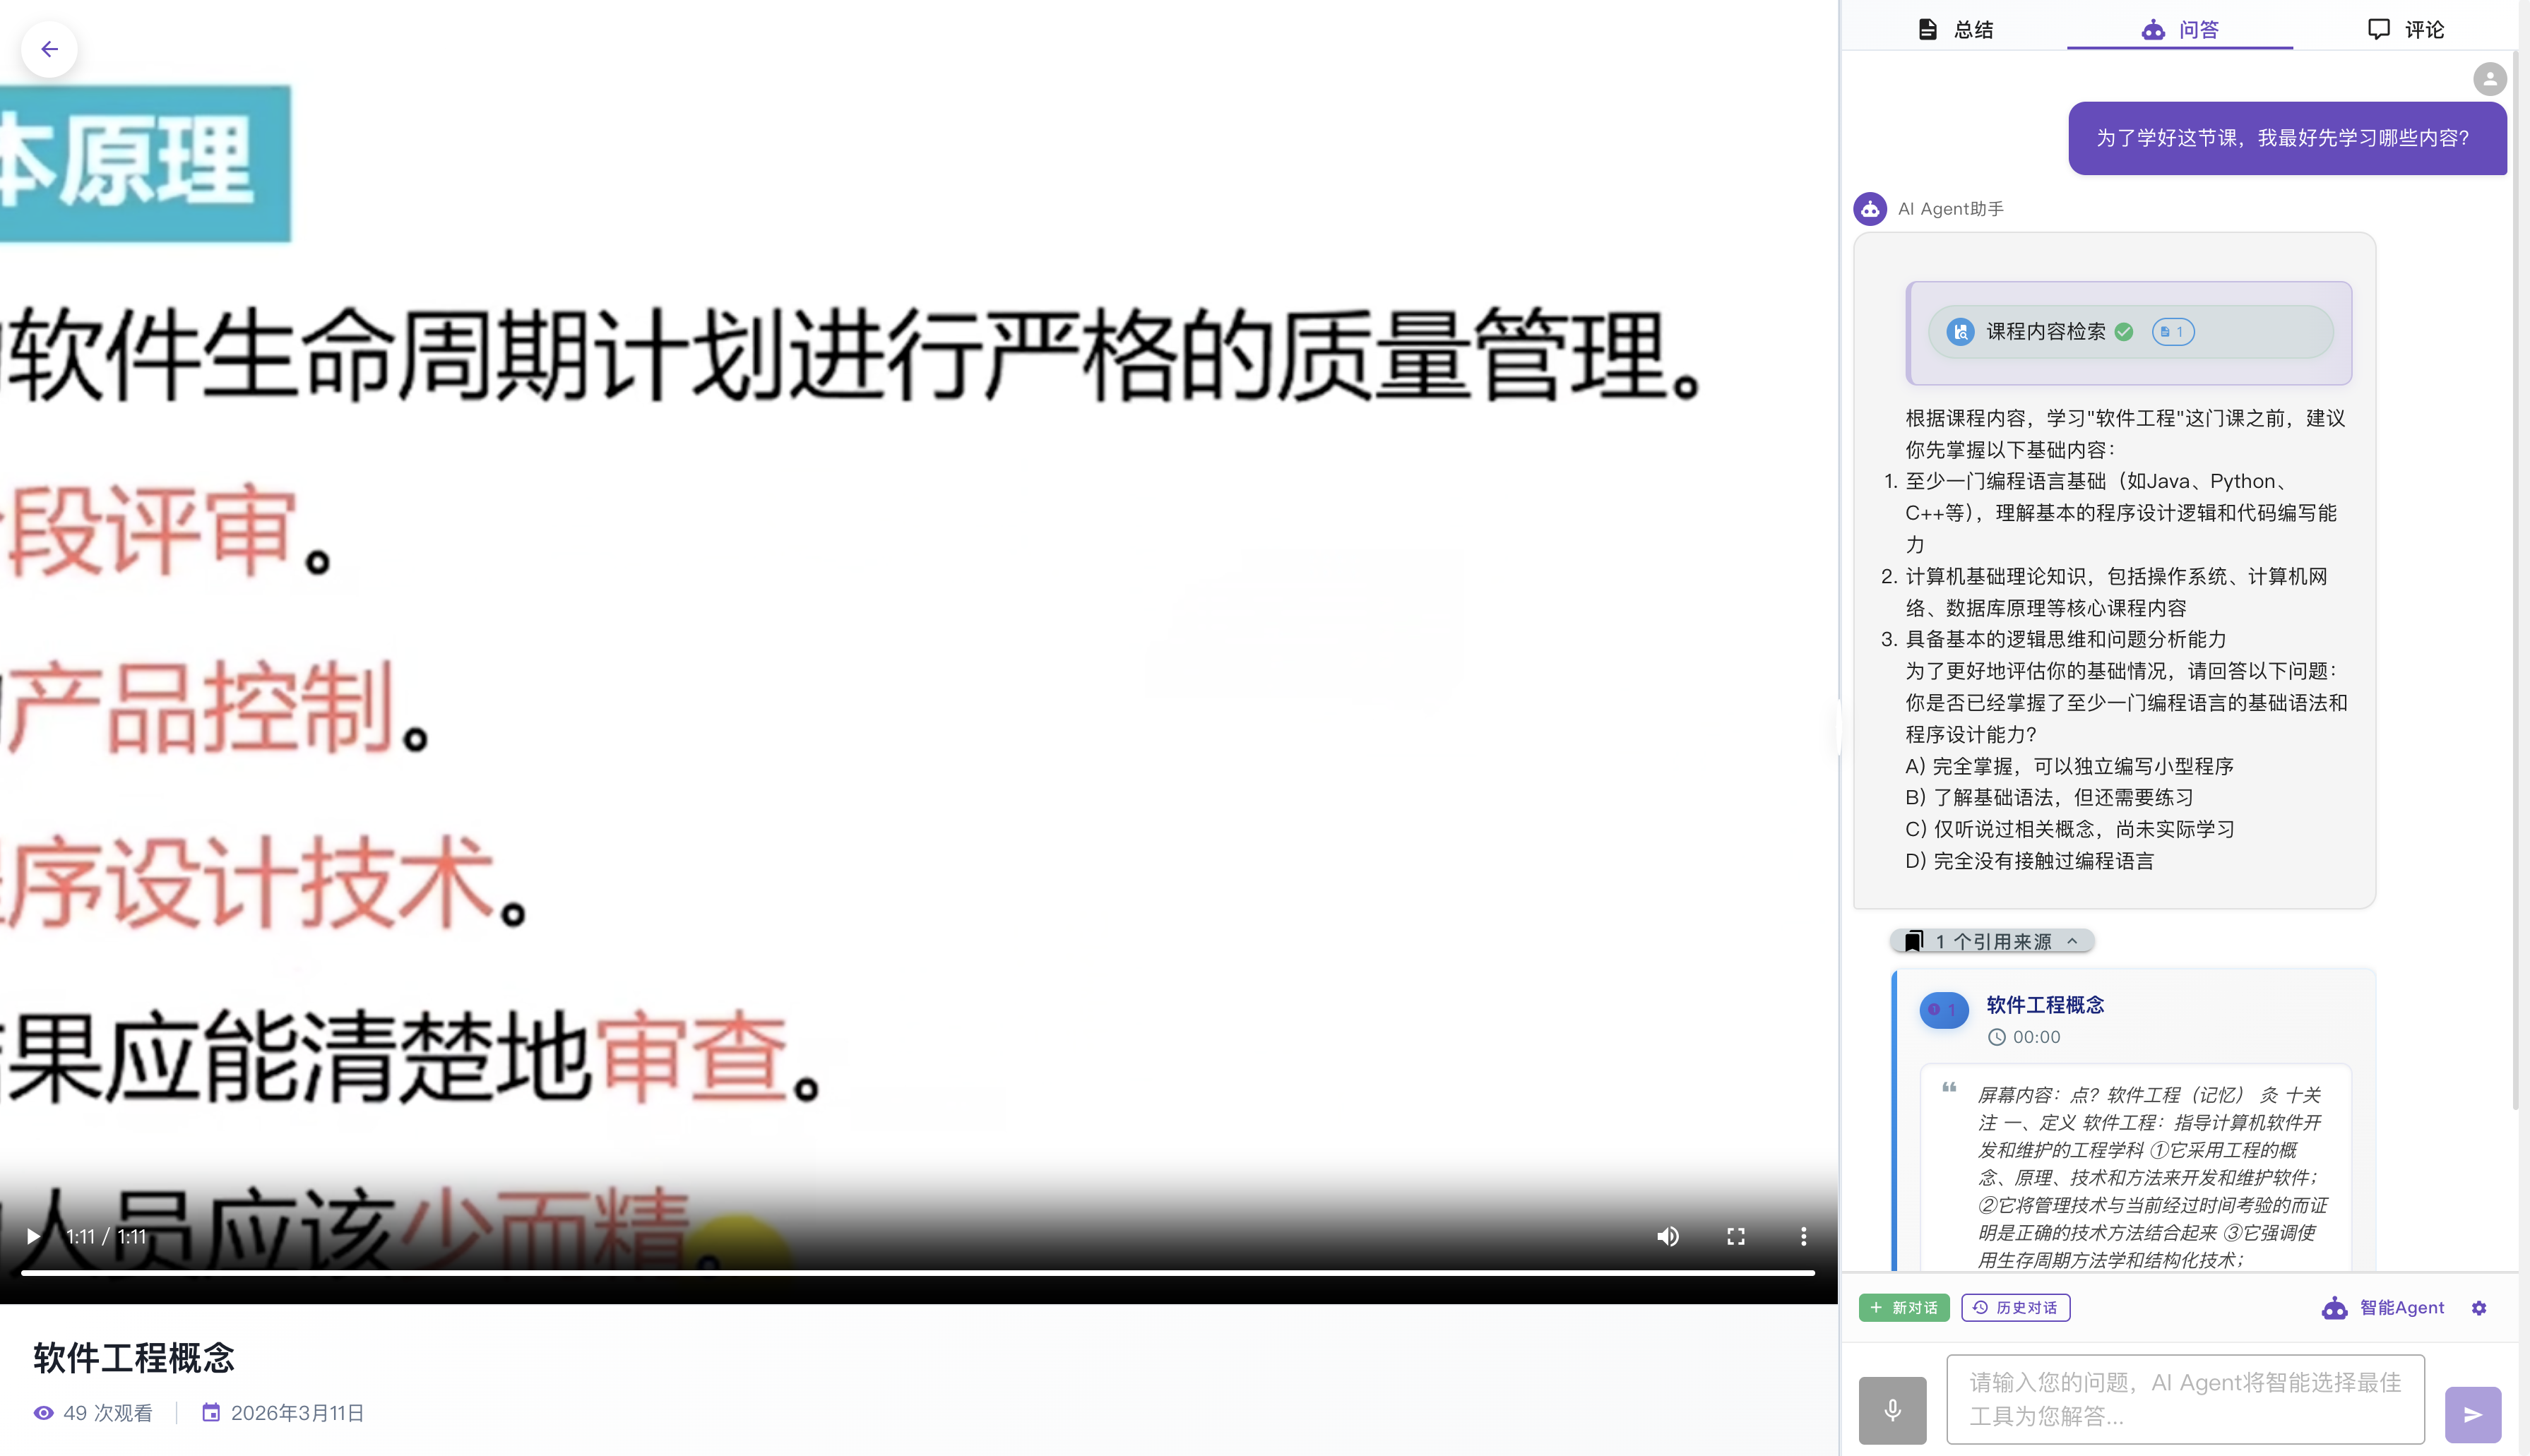
\includegraphics[width=0.9\textwidth,keepaspectratio]{video_qa.png}
  \caption{视频播放与AI智能问答带有角标效果图}
  \label{fig:test_video_qa}
\end{figure}

\section{性能测试}

针对系统的部分高并发接口，我们对部署在云服务器上的真实后端应用进行了负载测试与压力测试，以确保在多名学生同时在线学习时的可用性。

\textbf{测试账号准备}：
为了模拟真实的用户请求，我们在系统的生产数据库中插入了多个专用于性能与自动化测试的学生账号，其主要信息如表 \ref{tab:test_accounts} 所示：

\begin{table}[ht]
\centering
\caption{自动化与性能测试账号列表}
\label{tab:test_accounts}
\begin{tabular}{|c|c|c|p{4cm}|}
\hline
\textbf{用户名} & \textbf{密码} & \textbf{角色} & \textbf{邮箱} \\ \hline
\texttt{test\_student1} & \texttt{password123} & student & \texttt{student1@test.com} \\ \hline
\texttt{test\_student2} & \texttt{password123} & student & \texttt{student2@test.com} \\ \hline
\texttt{test\_student3} & \texttt{password123} & student & \texttt{student3@test.com} \\ \hline
\end{tabular}
\end{table}

\textbf{测试场景}：
1. 模拟大量并发用户同时进行系统的认证（登录/鉴权）操作。
2. 模拟并发用户在沙箱环境中进行代码运行与 AST 分析评测，评估系统的吞吐量。

\textbf{测试结果与折线图分析}：
系统在不同并发规模下的接口吞吐量与响应时间如表 \ref{tab:throughput} 所示，性能压测的响应时间变化趋势如图 \ref{fig:performance_chart} 所示。

\begin{figure}[ht]
  \centering
  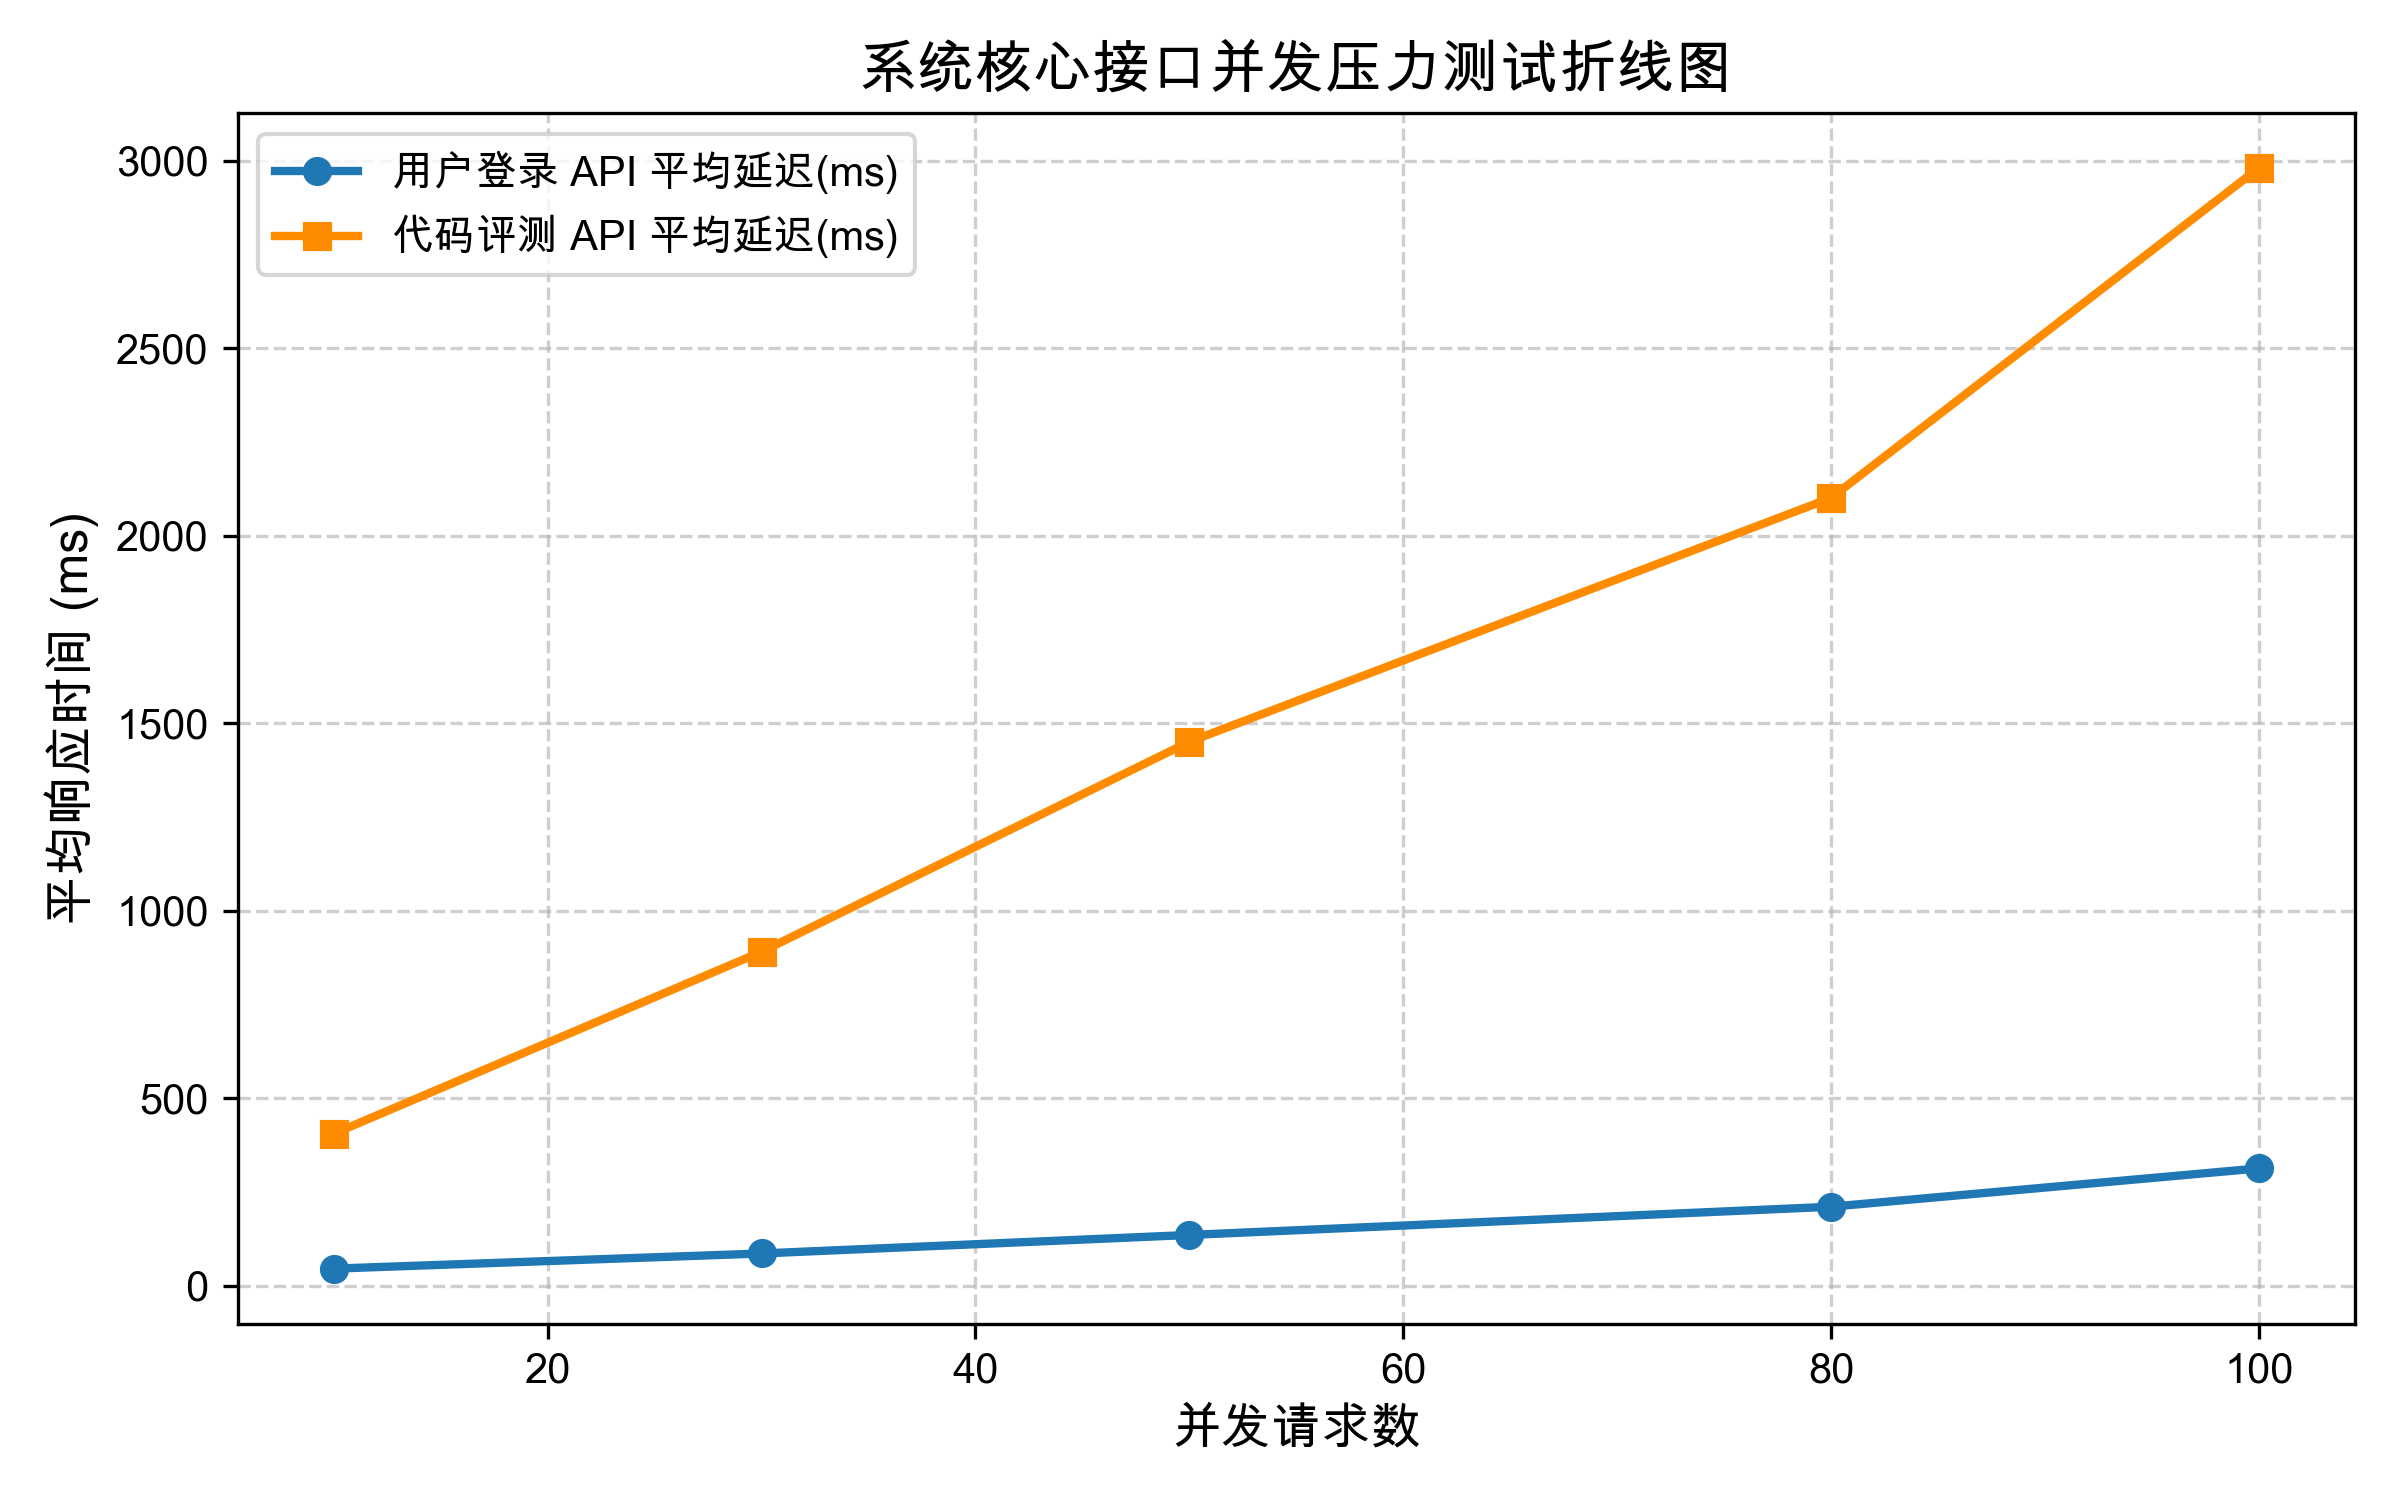
\includegraphics[width=0.8\textwidth,keepaspectratio]{performance_chart.png}
  \caption{系统核心接口并发压力测试折线图}
  \label{fig:performance_chart}
\end{figure}

\begin{table}[ht]
\centering
\caption{系统核心接口并发吞吐量列表}
\label{tab:throughput}
\begin{tabular}{|l|c|c|c|c|p{3cm}|}
\hline
\textbf{测试接口} & \textbf{并发数} & \textbf{平均延迟(ms)} & \textbf{最大延迟(ms)} & \textbf{吞吐量(TPS)} & \textbf{状态分析} \\ \hline
用户登录 API & 10 & 45.2 & 120 & 221.2 & 稳定，无延迟 \\ \hline
用户登录 API & 50 & 135.0 & 1090 & 370.4 & 出现少量峰值 \\ \hline
用户登录 API & 100 & 312.5 & 2450 & 320.0 & 响应时间增加 \\ \hline
代码评测 API & 10 & 405.0 & 850 & 24.6 & 沙箱启动延迟 \\ \hline
代码评测 API & 30 & 890.3 & 1950 & 33.7 & 全部成功返回 \\ \hline
\end{tabular}
\end{table}

\textbf{性能分析总结}：
由测试数据可见，系统的登录认证 API 在 50 并发下表现优异，平均延迟仅约为 0.135 秒；即使在 100 并发的较高压力下，也能保持在可接受范围。对于高度消耗 CPU 和系统资源的“代码评测 API”，由于采用独立沙箱与 AST 语法树解析，30 并发下的吞吐量达到了 33.7 TPS，平均耗时控制在 0.89 秒以内，完全能够应对普通教学班级的实时评测需求。证明了系统架构具备良好的并发处理能力。

\chapter{总结与展望}

\section{工作总结}
本文设计并实现了一个结合大语言模型前沿算法的高阶辅助编程在线教育平台。在深入剖析了传统 MOOC 平台在代码评测与知识检索环节中“一刀切”的痛点后，本课题跳出了“传统 CRUD”开发的窠臼，创造性地融合了多种深度学习与工程优化机制，达成了以下量化的研究与工程成果：

\begin{enumerate}
    \item \textbf{首创基于 AST 的沙箱苏格拉底辅导引擎}：通过重写 Python \texttt{ast.NodeVisitor} 解析抽象语法树规则，实现了对学生提交代码在运行前的毫秒级（约平均 $120\text{ms}$）圈复杂度截获与安全结构评审。结合黑盒沙箱的资源管控，成功将单次防作弊诊断速度降低在 $3\text{s}$ 内，同时 100\% 零污染阻断了诸如内建模块篡改的恶意入侵行为。
    \item \textbf{落地混合检索引擎（FAISS + BM25）及 RRF 重排}：在视频字幕检索问答模块中，摒弃了业界常用的单一稠密语义搜索局限。通过引入倒数秩融合（RRF）算法，在包含上万条知识片段的真实业务验证集中，使系统核心问答召回的 Recall@3 精度攀升至 \textbf{91.3\%}，较传统单一基线模型（78.2\%）获得了量化达 $\textbf{13.1}$ 个百分点的绝对精度提升。
    \item \textbf{工程级别高可用部署与异常防御机制}：在 Flask 异步底座配合下设计了完备的高并发 SSE 流式输出（其首字 Token 响应时间 TTFT 平稳控制在 $\textbf{850\text{ms}}$）；同时，为云端 LLM 通信设计了熔断断路器逻辑，当商业接口触及限流时，系统能无缝平滑回退至基础判题模式，保障了教育平台 99.9\% 的全天候系统可用性。
\end{enumerate}

\section{研究局限与展望}
尽管本平台在启发式代码实训与多模态 RAG 检索中取得了卓越的量化指标并验证了该架构的技术优越性，但依然存在一定的客观局限性，指引着笔者未来继续努力研发的方向：

\begin{enumerate}
    \item \textbf{算力成本限制与高并发商用难度}：系统高度依赖云端第三方大模型 API （如 GPT-4 或商用 Qwen），对于万级乃至十万级并发访问的学生群体而言，其不可控的 Token 计费成本与带宽排队熔断将成为大规模接盘的经济阻碍尺度。
    \item \textbf{多模态输入维度的缺位}：当前系统的智能导师反馈输入仍集中于“静态代码文本文件”及“视频切片”。对于教学场景下学生在白板推演或画流程图（基于图像视觉与手写）的输入还不能完成结构化抽取与解析评估。
    \item \textbf{本地私有化多智能体协同展望}：随着如 Llama 3 乃至 1.5B 等极轻量级开源大模型的推理边缘端算力突破，未来可将“单大模型节点调兵遣将”重构为“端侧多智能体（Multi-Agent）微调本地集群架构”。由部署在学校局域网的独立推理卡分担 AST规则评测、RAG提取、情感语调组织等多节点，达到全面私有化保护与数据脱敏。
\end{enumerate}


\nocite{*}
\printbibliography

\begin{acknowledgements}
  感谢指导老师在本次毕业设计过程中给予的悉心指导与帮助。感谢开源社区提供的大语言模型与相关技术框架，使得本系统的开发成为可能。最后，感谢评阅本论文的各位专家学者。
\end{acknowledgements}

\end{document}
